%-------------------------------------------------------------------------------------------
\documentclass[aspectratio=169,UTF8,11pt]{ctexbeamer}

%%%%%%%%%%%%%%%%%%%%%%%%%%%%%
\usepackage{colortbl}
\usepackage{color}
\usepackage{booktabs}
\usepackage{threeparttable}
\usepackage{hyperref}
%\usepackage{babel}
%%%%%%%%%%%%%%%%%%%%%%%%%%%%%

\mode<presentation> {
\usetheme{Madrid}
%\setbeamertemplate{footline} % To remove the footer line in all slides uncomment this line
\setbeamertemplate{footline}[frame number] % To replace the footer line in all slides with a simple slide count uncomment this line
\setbeamercolor{page number in head/foot}{fg=blue}
\setbeamertemplate{navigation symbols}{} % To remove the navigation symbols from the bottom of all slides uncomment this line
}

% User Defined Block %%%%%%%%%%%%%%%%%%%%%%%%%%%%%%%%%%%%%%%%%%%%%%%%%%%%%%%%
\usepackage{setspace}
\definecolor{orange}{rgb}{1,0.5,0}
\definecolor{aa}{RGB}{34,139,34}
\definecolor{lightblue}{rgb}{0,0.85,0.9}
\definecolor{darkblue}{rgb}{0,0.7,1}
\definecolor{hanblue}{rgb}{0.27, 0.42, 0.81}
\definecolor{indiagreen}{rgb}{0.07, 0.53, 0.03}
\definecolor{indianred}{rgb}{0.8, 0.36, 0.36}
\definecolor{indianyellow}{rgb}{0.89, 0.66, 0.34}
\definecolor{babypink}{rgb}{0.96, 0.76, 0.76}
\definecolor{ao(english)}{rgb}{0.0, 0.5, 0.0}
\definecolor{bondiblue}{rgb}{0.0, 0.58, 0.71}
\definecolor{ao(english)}{rgb}{0.0, 0.5, 0.0}
\definecolor{azure(colorwheel)}{rgb}{0.0, 0.5, 1.0}
\setbeamerfont{block title}{size=\normalsize}
\setbeamerfont{block body}{size=\small}

% User Defined Block %%%%%%%%%%%%%%%%%%%%%%%%%%%%%%%%%%%%%%%%%%%%%%%%%%%%%%%%
\newenvironment<>{abstractblock}[1]{%
  \setbeamercolor{block title}{fg=white,bg=bondiblue}%
%   \setbeamercolor{block body}{fg=white,bg=bondiblue}%
  \begin{block}#2{#1}}{\end{block}}
\newenvironment<>{blueblock}[1]{%
  \setbeamercolor{block title}{fg=white,bg=hanblue}%
  \begin{block}#2{#1}}{\end{block}}

\newenvironment<>{greenblock}[1]{%
  \setstretch{1.3}\setbeamercolor{block title}{fg=white,bg=indiagreen}%
  \begin{block}#2{#1}}{\end{block}}

\newenvironment<>{redblock}[1]{%
  \setstretch{1.3}\setbeamercolor{block title}{fg=white,bg=indianred}%
  \begin{block}#2{#1}}{\end{block}}

\newenvironment<>{yellowblock}[1]{%
  \setstretch{1.3}\setbeamercolor{block title}{fg=white,bg=indianyellow}%
  \begin{block}#2{#1}}{\end{block}}

%----------------------------------------------------------------------------------------
%	PACKAGES
%----------------------------------------------------------------------------------------
\usepackage{graphicx} % Allows including images
%\usepackage{tikz}
%\usetikzlibrary{shapes.geometric, arrows}
\usepackage{listings}
\lstset{language=C++,
    columns=flexible,
   % basicstyle=\scriptsize\ttfamily,                                      % 设定代码字体、大小4
    basicstyle=\footnotesize\ttfamily,
    %numbers=left,xleftmargin=2em,framexleftmargin=2em,                   % 在左侧显示行号
    %numberstyle=\color{darkgray},                                        % 设定行号格式
    keywordstyle=\color{blue},                                            % 设定关键字格式
    commentstyle=\color{ao(english)},                                     % 设置代码注释的格式
    stringstyle=\color{brown},                                            % 设置字符串格式
    %showstringspaces=false,                                              % 控制是否显示空格
	%frame=lines,                                                         % 控制外框
    breaklines,                                                           % 控制是否折行
    postbreak=\space,                                                     % 控制折行后显示的标识字符
    breakindent=5pt,                                                      % 控制折行后缩进数量
    emph={size\_t,array,deque,list,map,queue,set,stack,vector,string,pair,tuple}, % 非内置类型
    emphstyle={\color{teal}},
    escapeinside={(*@}{@*)},
    literate={&}{{\color{red}\&}}{1}                                      %{<replace>}{<replacement text>}{<length>} no comma between items
}

\usepackage{tikz}
%---------------------------------------------------------------------------------------------------

%%%%%%%%%%%%%%%%%%%%%%%%%%%%%%%%%%%%%%%%%%%%%%%%%%%%%%%%%%%%%%%%%%%%%%%%%%%%%%%%%%%%%%%%%%%%%%
\title[\textit{面向对象程序设计 }]{面向对象程序设计-课程介绍}
\author[李长河]{李长河} % Your name
\institute[CUG] % Your institution as it will appear on the bottom of every slide, may be shorthand to save space
{
中国地质大学(武汉)自动化学院\\ % Your institution for the title page
\medskip
\textit{lichanghe@cug.edu.cn} % Your email address
}
\date{} % Date, can be changed to a custom date
%%%%%%%%%%%%%%%%%%%%%%%%%%%%%%%%%%%%%%%%%%%%%%%%%%%%%%%%%%%%%%%%%%%%%%%%%%%%%%%%%%%%%%%%%%%%%%

%-----------------------------------------------------------



\begin{document}

\maketitle
%-----------------------------------------------------------
\begin{frame}

	\begin{block}{课程简介}
	本课程是中国地质大学(武汉)面向信息类相关专业开设的一门公共基础课,授课对象为本科一年级和二年级学生。讲解C++语言程序设计方法。

	\end{block}
	\begin{block}{课程目标}
    \begin{itemize}
      \item 掌握计算机综合程序设计方法,建立\alert{编程思维};
      \item 具有扎实的C/C++语言基础,掌握基于对象、\alert{面向对象、泛型编程}等编程方法;
      \item 能够运用基本\alert{数据结构和算法}解决复杂问题,掌握\alert{可视化软件开发}技术;
      \item 具有综合系统分析、设计和实现能力,理论知识和编程能力达到\alert{高级程序员}水平。
    \end{itemize} 	
	\end{block}
\end{frame}

%-----------------------------------------------------------
\begin{frame}
\begin{columns}
	\begin{column}{0.55\textwidth}
\begin{block}{我国软件产业现状}
\begin{itemize}
  \item 软件业价值失衡导致产业\alert{大而不强}。“重硬轻软”,软件价值认证体系不健全;
  \item \alert{核心技术缺失}制约软件高质量发展。聚焦于应用创新而非核心技术的掌握;
  \item 面向重要行业的\alert{基础软件、高端软件供给不足}。例如操作系统、数据库、CAD软件、MatLab;
  \item 软件国际市场影响力和竞争力相对落后;
  \item 人才结构失衡的影响日益凸显等问题突出。人工智能、大数据、区块链、工业互联网等新兴产业人才需求缺
口逐步扩大,\alert{基础编程人才紧缺}。
\end{itemize}
\end{block}

	\end{column}
	\hfill
	\begin{column}{0.45\textwidth}
		
		\begin{tabular}{l}
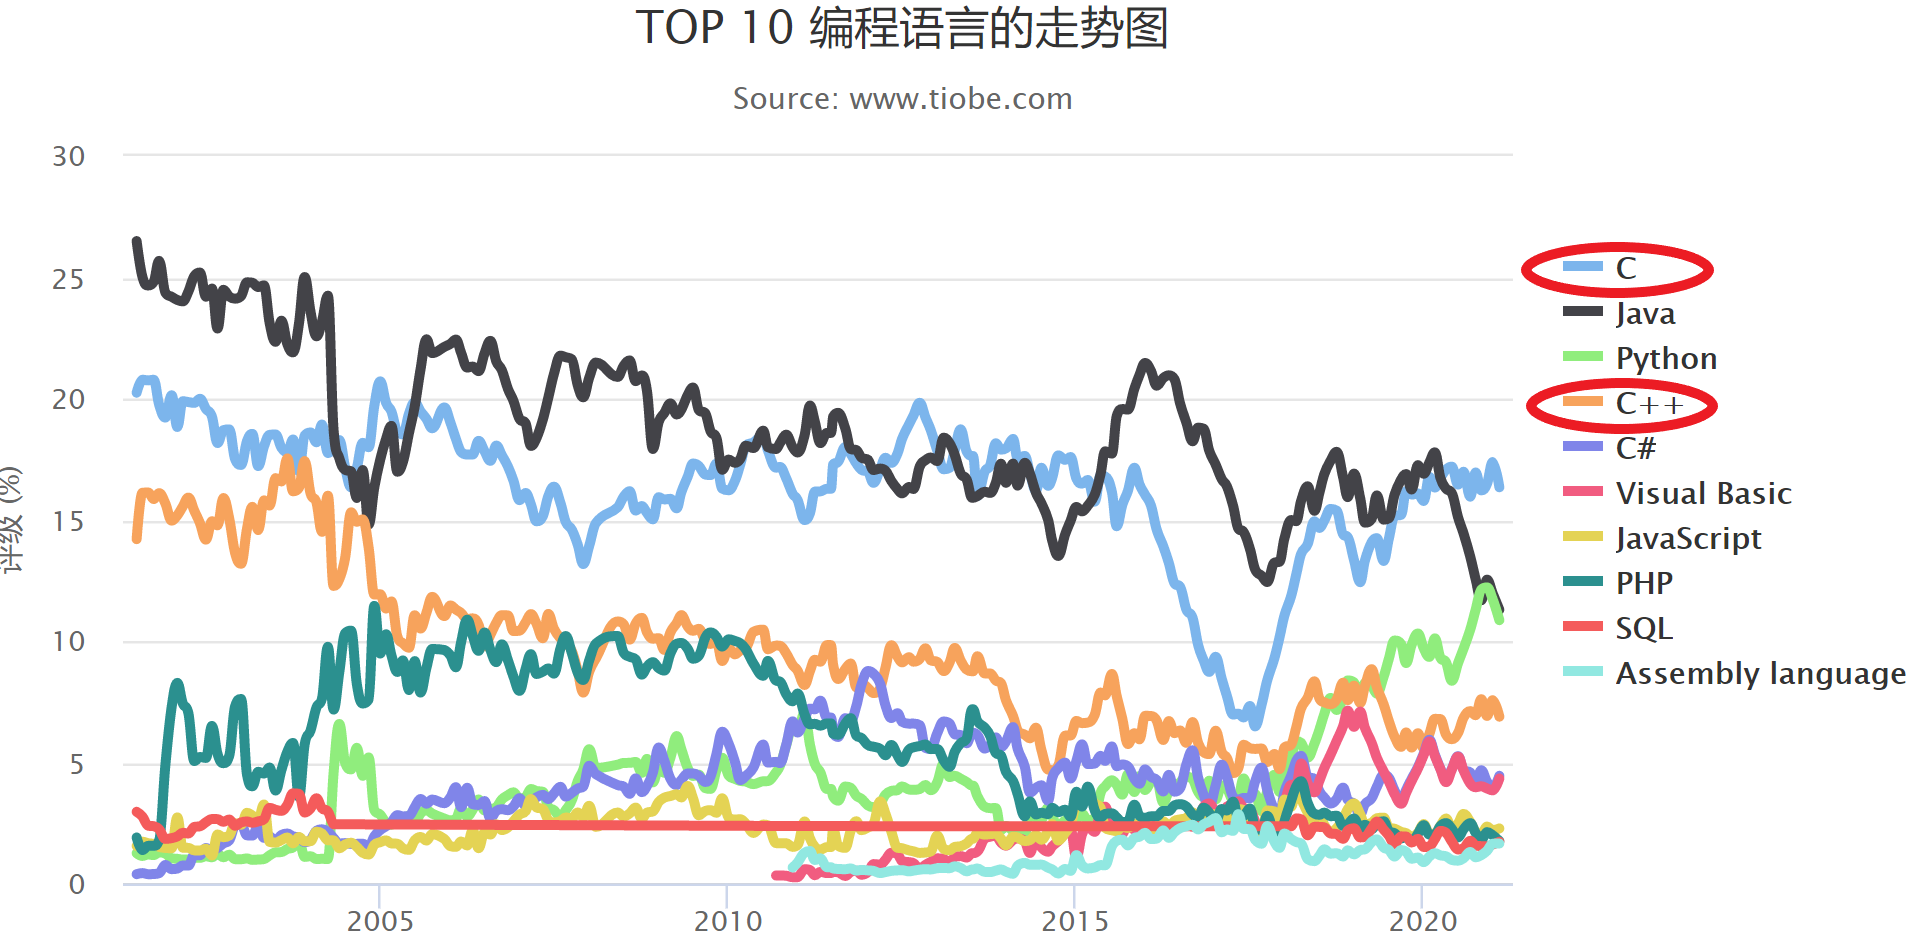
\includegraphics[scale=0.13]{排名变化.png}\\
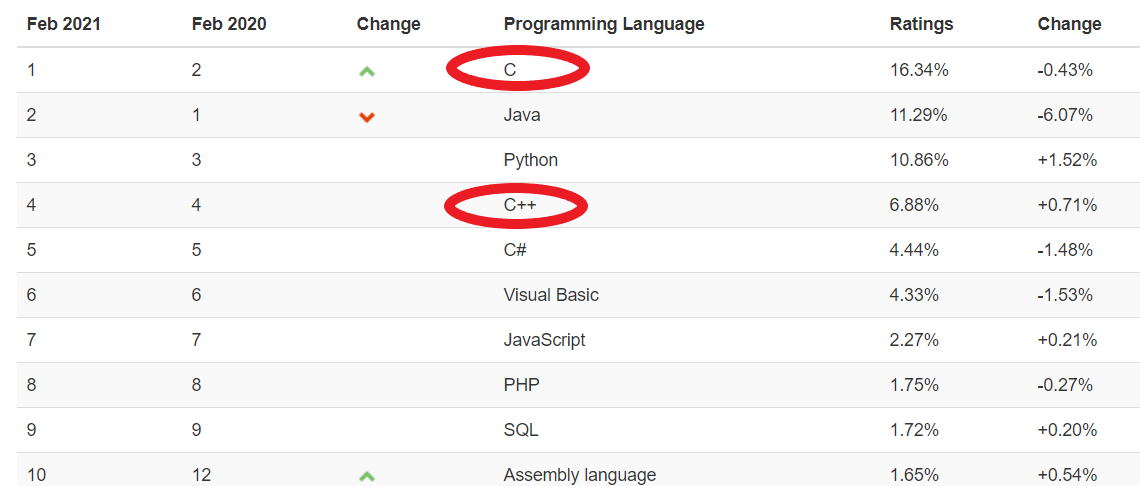
\includegraphics[scale=0.2]{最新排名.png}
		\end{tabular}
	\end{column}
\end{columns}
\end{frame}

%-----------------------------------------------------------
\begin{frame}
\begin{columns}
	\begin{column}{0.65\textwidth}
	\begin{block}{教材与实验指导书}
    \begin{itemize}
      \item 李长河, 童恒建, 叶亚琴等, C++程序设计(基于C++11标准). 电子工业出版社, 2019年10月第3次印刷
      \item 李长河, 刘小波, 徐迟等, C++程序设计实验指导书(基于C++11标准). 中国地质大学出版社,2020年12月
    \end{itemize}
	\end{block}
\begin{block}{电子资源}
{\footnotesize \url{https://github.com/Changhe160/cplusplus2020-2021-2}} \\
	\end{block}
\begin{block}{参考书}
	Stanley B. Lippman,Jos\'{e}e Lajoie,Barbara E. Moo.C++ Primer(第五版).王刚等译.北京:电子工业出版社,2013.	
	\end{block}
	\end{column}
	\hfill
	\begin{column}{0.3\textwidth}
	\begin{tabular}{c}
	
\includegraphics[scale=0.5]{book.jpg}\\
    
\includegraphics[scale=0.065]{C++实验指导书.png}
	\end{tabular}
	\end{column}
\end{columns}
\end{frame}

%-----------------------------------------------------------
\begin{frame}
\begin{block}{课程纪律}
\begin{enumerate}
\item 线下课堂上严禁看手机;
\item 课下作业和上机考试严禁抄袭,一经发现,均记0分处理。
\end{enumerate}
\end{block}

\begin{block}<2->{课下要求}
\begin{itemize}
  \item 动手是前提,每个星期保证独立上机完成1-2个程序的调试;
  \item 学会课外找资料(上网或翻阅书籍)解决问题;
  \item 交流和探讨;
\end{itemize}
\end{block}
\begin{block}<3->{课时安排}
讲课学时:16,课内实验学时:16,课外实验:16
\end{block}
\begin{block}<4->{实验安排}
4次上机考试,时间地点待定
\end{block}

\end{frame}

%-----------------------------------------------------------
\begin{frame}
\begin{columns}
\column{0.55\textwidth}
\begin{block}{课程考核}
总成绩 = 考勤*5\%+四次上机考核*40\%+1次综合考核*40\%+ 课程报告*15\%\\
考核方式:线上提交+线上/线下验收\\
提交系统:操作指南见电子资源主页\\
\url{http://course.educg.net/indexcs/simple.jsp?loginErr=0}
\end{block}
\begin{block}{课程群}
  QQ群:940393564\\
  助教:杨瑞
\end{block}
\column{0.45\textwidth}
\begin{center}
  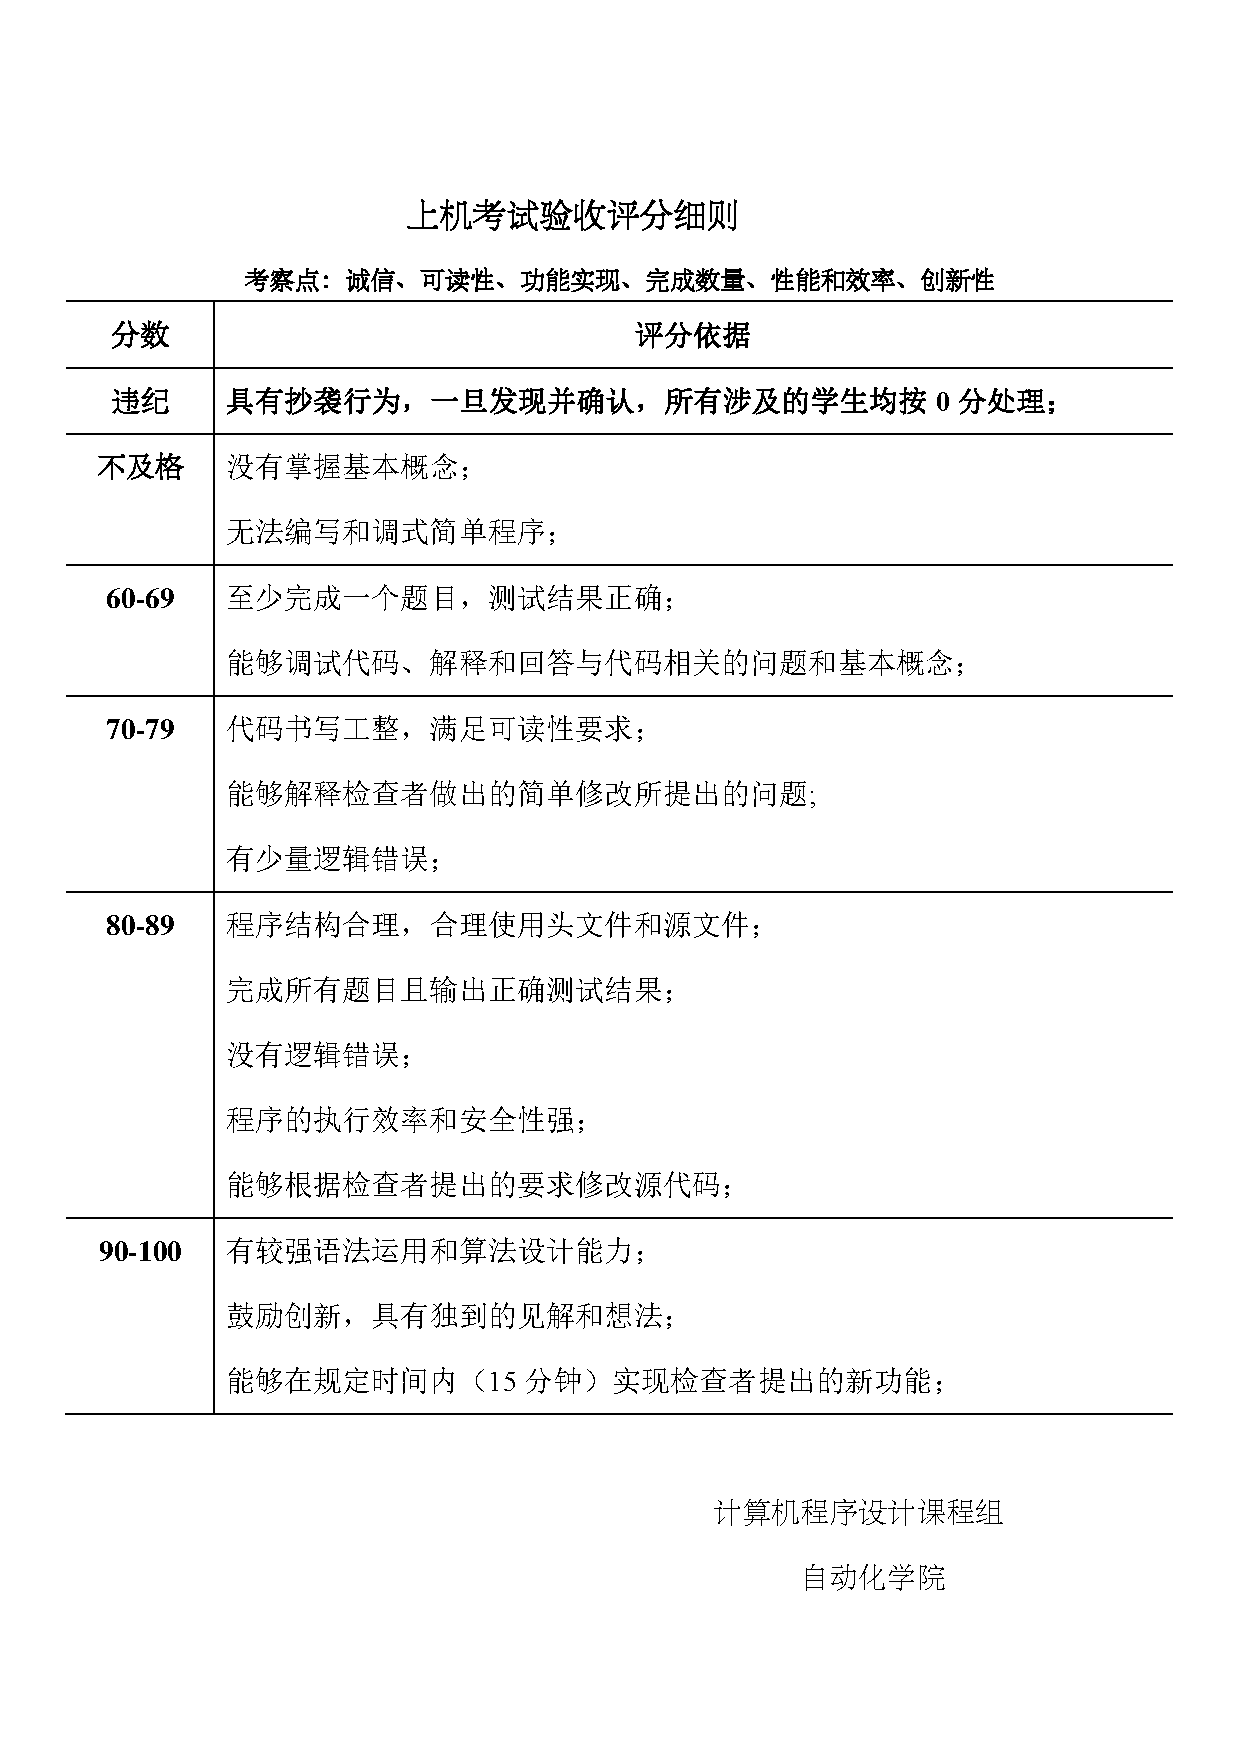
\includegraphics[scale=0.3]{上机考核评分依据.pdf}
\end{center}
\end{columns}
\end{frame}

\end{document}
